\documentclass[tikz, border=10pt]{standalone}
\usetikzlibrary{arrows.meta}

\begin{document}
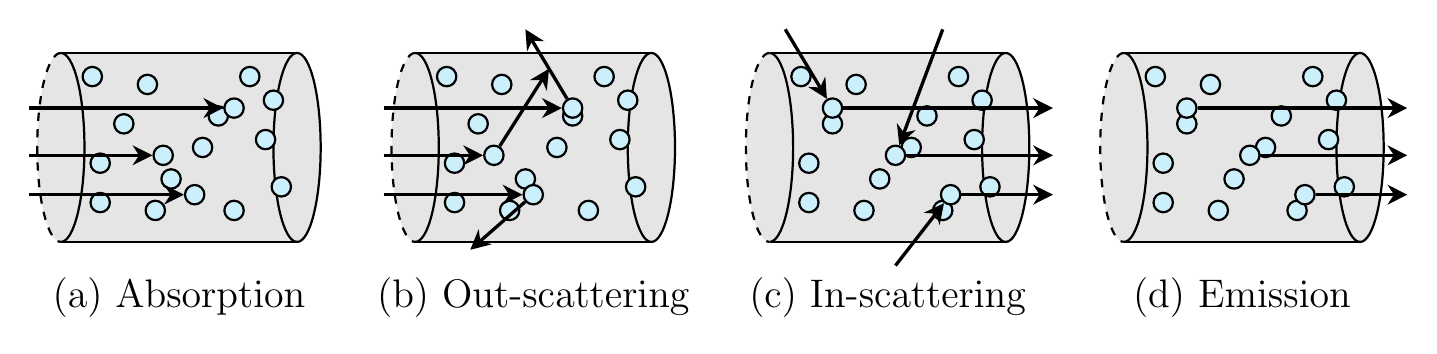
\begin{tikzpicture}[
    % Style for the particles (light blue circles)
    p/.style={circle, draw=black, thick, fill=cyan!20, inner sep=0pt, minimum size=7pt},
    % Style for the light rays (arrows)
    ray/.style={-{Stealth[length=2.5mm, width=2.5mm]}, very thick}
]

% Macro to draw the 3D-looking cylinder background
\newcommand{\drawcylinder}{
    % Fill inner volume and ellipses with light gray
    \fill[black!10] (0,1.2) -- (3.0,1.2) -- (3.0,-1.2) -- (0,-1.2) -- cycle;
    \fill[black!10] (0,0) ellipse (0.3 and 1.2);
    \fill[black!10] (3.0,0) ellipse (0.3 and 1.2);
    
    % Draw back of left ellipse (dashed to show it's hidden)
    \draw[thick, dashed] (0,1.2) arc (90:270:0.3 and 1.2);
    % Draw front of left ellipse (solid)
    \draw[thick] (0,-1.2) arc (-90:90:0.3 and 1.2);
    
    % Draw top and bottom boundaries of the cylinder
    \draw[thick] (0,1.2) -- (3.0,1.2);
    \draw[thick] (0,-1.2) -- (3.0,-1.2);
    
    % Right ellipse (fully solid as it's facing us)
    \draw[thick] (3.0,0) ellipse (0.3 and 1.2);
}

% Macro to scatter some random background particles
\newcommand{\bgparticles}{
    \node[p] at (0.4, 0.9) {};
    \node[p] at (1.1, 0.8) {};
    \node[p] at (2.4, 0.9) {};
    \node[p] at (2.7, 0.6) {};
    \node[p] at (0.8, 0.3) {};
    \node[p] at (2.0, 0.4) {};
    \node[p] at (0.5, -0.2) {};
    \node[p] at (1.8, 0.0) {};
    \node[p] at (2.6, 0.1) {};
    \node[p] at (0.5, -0.7) {};
    \node[p] at (1.4, -0.4) {};
    \node[p] at (2.2, -0.8) {};
    \node[p] at (2.8, -0.5) {};
    \node[p] at (1.2, -0.8) {};
}

% ==========================
% (a) Absorption
% ==========================
\begin{scope}[shift={(0,0)}]
    \drawcylinder
    \bgparticles
    
    % Target Particles
    \node[p] (a1) at (2.2, 0.5) {};
    \node[p] (a2) at (1.3, -0.1) {};
    \node[p] (a3) at (1.7, -0.6) {};
    
    % Incoming Rays terminating at particles
    \draw[ray] (-0.4, 0.5) -- (a1);
    \draw[ray] (-0.4, -0.1) -- (a2);
    \draw[ray] (-0.4, -0.6) -- (a3);
    
    \node[font=\rmfamily\Large] at (1.5, -1.9) {(a) Absorption};
\end{scope}

% ==========================
% (b) Out-scattering
% ==========================
\begin{scope}[shift={(4.5,0)}]
    \drawcylinder
    \bgparticles
    
    % Target Particles
    \node[p] (b1) at (2.0, 0.5) {};
    \node[p] (b2) at (1.0, -0.1) {};
    \node[p] (b3) at (1.5, -0.6) {};
    
    % Outgoing scattered rays (drawn first so arrows sit cleanly)
    \draw[ray] (b1) -- ++(-0.6, 1.0);  % Scatters up-left
    \draw[ray] (b2) -- ++(0.7, 1.1);   % Scatters up-right
    \draw[ray] (b3) -- ++(-0.8, -0.7); % Scatters down-left
    
    % Incoming straight rays
    \draw[ray] (-0.4, 0.5) -- (b1);
    \draw[ray] (-0.4, -0.1) -- (b2);
    \draw[ray] (-0.4, -0.6) -- (b3);
    
    \node[font=\rmfamily\Large] at (1.5, -1.9) {(b) Out-scattering};
\end{scope}

% ==========================
% (c) In-scattering
% ==========================
\begin{scope}[shift={(9.0,0)}]
    \drawcylinder
    \bgparticles
    
    % Target Particles
    \node[p] (c1) at (0.8, 0.5) {};
    \node[p] (c2) at (1.6, -0.1) {};
    \node[p] (c3) at (2.3, -0.6) {};
    
    % Outgoing straight rays aligned horizontally
    \draw[ray] (c1) -- (3.6, 0.5);
    \draw[ray] (c2) -- (3.6, -0.1);
    \draw[ray] (c3) -- (3.6, -0.6);
    
    % Incoming scattered rays from angles
    \draw[ray] (0.2, 1.5) -- (c1);  
    \draw[ray] (2.2, 1.5) -- (c2);  
    \draw[ray] (1.6, -1.5) -- (c3); 
    
    \node[font=\rmfamily\Large] at (1.5, -1.9) {(c) In-scattering};
\end{scope}

% ==========================
% (d) Emission
% ==========================
\begin{scope}[shift={(13.5,0)}]
    \drawcylinder
    \bgparticles
    
    % Target Emitting Particles
    \node[p] (d1) at (0.8, 0.5) {};
    \node[p] (d2) at (1.6, -0.1) {};
    \node[p] (d3) at (2.3, -0.6) {};
    
    % Outgoing rays originating from particles
    \draw[ray] (d1) -- (3.6, 0.5);
    \draw[ray] (d2) -- (3.6, -0.1);
    \draw[ray] (d3) -- (3.6, -0.6);
    
    \node[font=\rmfamily\Large] at (1.5, -1.9) {(d) Emission};
\end{scope}

\end{tikzpicture}
\end{document}